\nisar{todo: remove giant whitespaces from eqs. and figs. } In the following derivations and explanations of \xO{} and \xQ{}, the following symbols will be used: the bar symbol ($\bar{y}$) indicates a reference value; star ($y^*$) indicates an optimum; tilde ($\tilde{y}$) symbol indicates an approximate or simulated quantity (i.e. via Monte-Carlo); and hat ($\^{y}$) symbol indicates a predicted quantity (i.e. from a surrogate model). Quantities without these modifiers can be considered to be generic or theoretical/true values.

\subsection{Outcome Assessment Definition and Calculation} \label{sec:xO}
An approach for computing \xO{} was developed in \cite{Aitken2016-cv} for infinite horizon MDPs. First, begin with the following assumptions: $\xM=\xMup$ (perfectly known problem/task model), $\xI= \xIup$ (perfectly interpreted user task command and reward function $R_k$), $\xQ=\xQup$ (optimal policy \piopt{} known and available), and $\xP=\xPup$ (task encountered previously) \nisar{need to rethink using numbers for these here -- suffices to say that we are in boundary conditions where these don't affect \xO{} -- then also need to revisit this in discussion or remark that idea is similar to conditional indep. of factors -- future work will hierarchically relax assumptions...}. Under these conditions, overall self-confidence depends only on \xO{}, which can then be quantified as a measure of the probability distribution  $\rwdopt = \ppioptri$ of achievable \nisar{should be `discounted', by $\gamma$?} cumulative reward values $\ri= \sum_{k=0}^{\infty}R_{k}$ under policy \piopt. \nisar{for me to redo: need to rethink this way of explaining connection to $\rwdopt$..is there a more principled connection via concept of meta-analysis? [refs?] }. 

\nisar{should go a bit earlier?} Intuitively, \rwdopt{} summarizes the landscape of possible outcomes for the APS if it were to apply the policy \piopt{} to carry out its task, and thus provides useful information about the intrinsic difficulty or feasibility of a task beyond just the mean value of \ri{} (which \piopt{} maximizes via an MDP solver). For instance, if a significant portion of the probability mass in \rwdopt{} concentrates around very large negative values, then the task cannot be achieved without a high probability of encountering unfavorable outcomes (even with optimal decision-making). 

Along these lines, ref. \cite{Aitken2016-cv} considers several measures of \rwdopt, including the logistically transformed upper partial moment/lower partial moment (UPM/LPM) score given in Eq.~\ref{eq:upm_lpm}, which quantifies how much probability mass lies to the right vs. left of a reference minimally acceptable cumulative reward value \ris{} (e.g. any reward greater than 0 is acceptable).
    \begin{align}
        \frac{UPM}{LPM}\left(p,\riref\right) &= \frac{\int_{\riref}^{+\infty}zp(z)dz}{\int_{-\infty}^{\riref} zp(z)dz} \label{eq:upm_lpm}
    \end{align}

In the Donut Delivery problem, \riref{} is the reward obtained at a user-specified maximum acceptable time to successfully reach the delivery destination. The distribution $p = \rwdoptapprox$ is empirically estimated from Monte Carlo sample simulations of \rwdopt, by applying \piopt{} to the assumed MDP state dynamics model.

The range of UPM/LPM is unbounded (i.e. $(-\infty,+\infty)$)) and so cannot be easily or accurately interpreted by humans. Because of this, \xO{} is a logistically transformed, scaled, and shifted version of UPM/LPM, so that the value lies on the range $[-1,+1]$, 
    \begin{align}
        \xO &= \frac{2}{1+e^{-\log\left(\frac{UPM}{LPM}\right)}}-1 \label{eq:xO}
    \end{align}
    \begin{figure}[tbp]
        \centering
        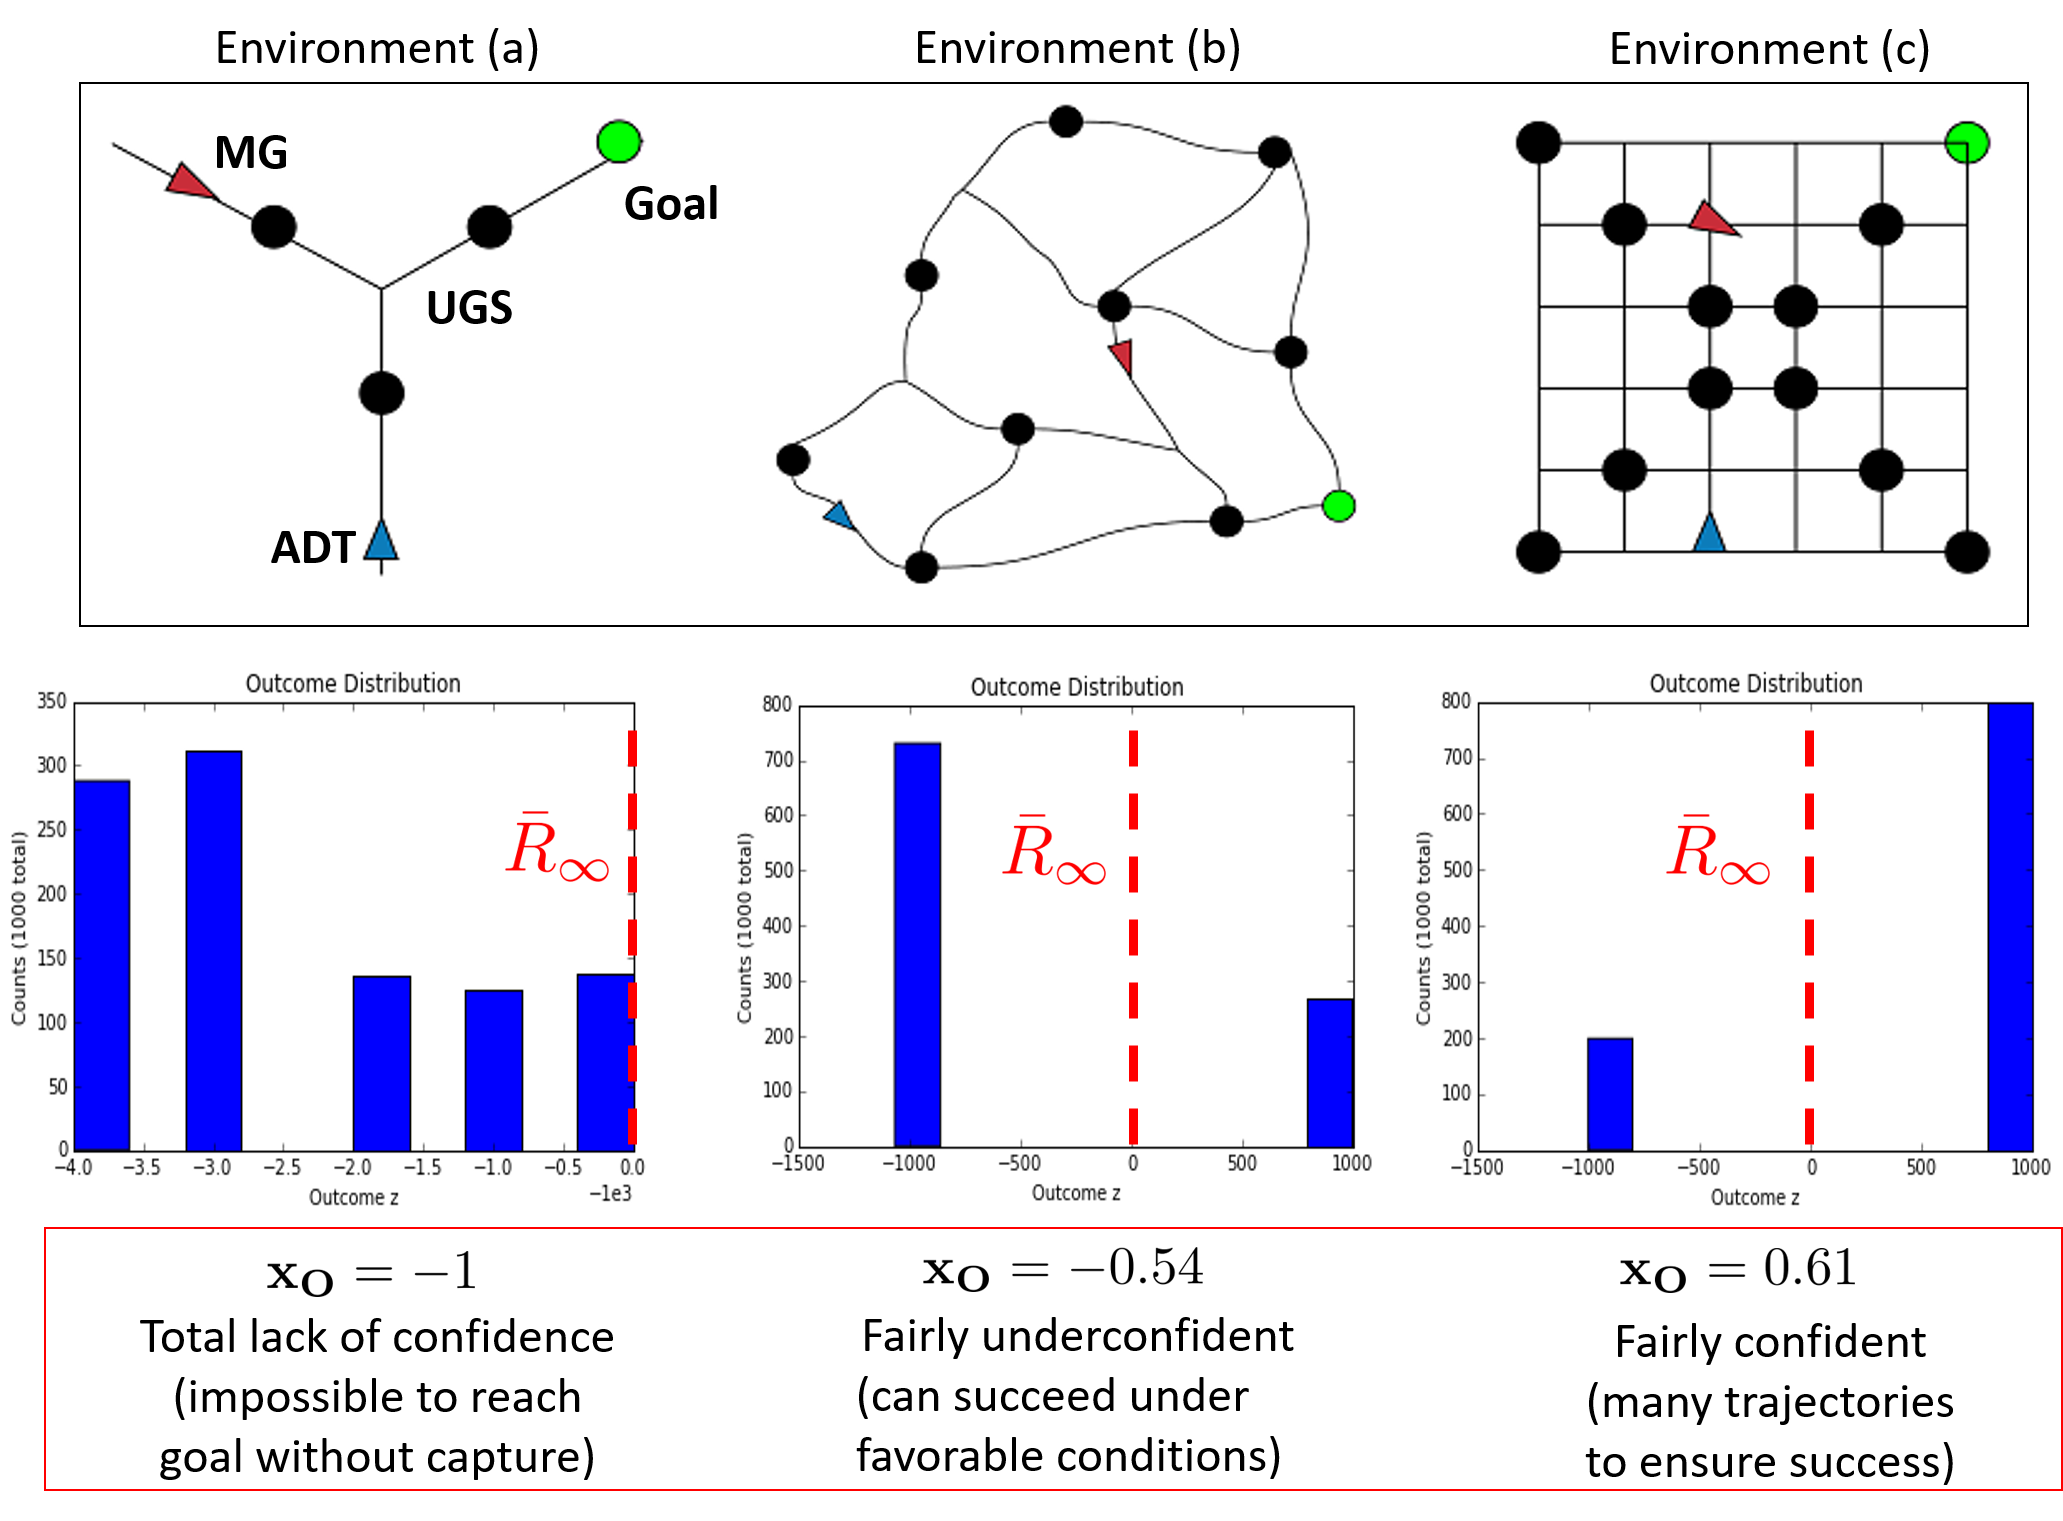
\includegraphics[width=0.95\linewidth]{Figures/xO_EnvsRewardsOnly.png}
        \caption{\xO{} assessments for Donut Delivery problem in various environments. \nisar{get rid of left half of fig., expand plots}}
        \label{fig:xOexample}
        \vspace{-0.5 cm}
    \end{figure}
\noindent Fig.~\ref{fig:xOexample} illustrates the resulting value of \xO{} in three different situations. In `Environment (a)' the acceptable reference reward \ris{} is on the far right side of the distribution, and all of the probability mass is left of it, resulting in $\xO=0$. In the other two examples \ris{} is in the middle of the distributions, but due to higher probability mass being left or right \xO{} changes sign. This assessment of the predicted outcomes given the APS the capability to communicate its capabilities and limitations with users.

\subsection{Solver Quality Definition and Calculation} \label{sec:xQ}
In the context of APS planning, \xQ{} indicates how well a generic solver \solve{} for a planning problem will `perform' on a given task \task{} of class \taskclass{}. This work restricts \taskclass{} to the class of all applicable MDP problems, so that \solve{} is any type of MDP solver  (although the ideas developed here can in principle be easily extended beyond MDPs or planning problems alone).

A formal definition for \xQ{} must make the notion of \solve{}'s `performance' precise to enable some form of quantitative evaluation. For MDPs, any particular task instance \task{} has a corresponding optimal policy \piopt{} which by definition leads to corresponding best achievable total reward. This suggests that a natural performance metric for assessing the competence of a generic solver \solve{} would be some quantitative comparison of the (not necessarily optimal) policy \pigeneric{} to \piopt. Such a `strong' comparison can be done in many ways depending on the application context, e.g. by directly comparing actions taken by the policies in different states of interest, or by comparing the resulting expected total reward distributions or other artifacts of the different policies. 
But since \piopt{} is usually unavailable (or else \solve{} would not be needed), \xQ{} should also allow for `weak' comparison to other reference `baseline' solvers that yield policies with performance as good as/very close to the true optimal \piopt. This may require comparing two completely different types of solvers (e.g. a deterministic approximation vs. a Monte Carlo approximation), so \xQ{} should also ideally enable comparison across solver classes, as well as assessments of online/anytime solvers (for which complete state coverage and policy convergence may not be possible in large state/action spaces).
 
At the same time, \xQ{} should account for the expected self-confidence metric trends and boundary conditions mentioned earlier in Fig. \ref{fig:trendsBCs} for the Donut Delivery application. In particular, \xQ{} should be defined also to naturally account for the influence of both characteristics of \solve{} and features of \task{} simultaneously. For instance, if the task \task{} is not particularly complex or is characterized by a very small amount of uncertainty (e.g. so as to be nearly deterministic), then it is possible that \brett{does this make sense?--} a small sample size could suffice to closely approximate the optimal policy, in which case \xQ{} should indicate very high confidence. Moreover, while it is impossible to assess performance on \emph{all} tasks in \taskclass{}, \xQ{} should be able to reflect \solve{}'s performance on \emph{any} task instance \task{} in \taskclass{}, including previously unseen tasks (e.g. new road networks for the Donut Delivery problem). 

A natural starting point for devising a quantitative assessment of \xQ{} according to these desiderata is to again examine how information about \rwdapprox{} (which is already used to form \xO{}) can be analyzed further. 
Note that \xO{} indirectly depends on \xQ{}, since reliable estimation of \rwdoptapprox{} requires knowing the optimal policy \piopt. But in practice, an MDP-based APS will often employ an approximate policy \piapprox{} instead of the true optimal policy \piopt. In turn, this leads to an estimate \rwdapprox{} of the expected reward distribution which differs from the true \rwdopt{} under the optimal \piopt.

\brett{This segue is important, need to re-check this:} We show next that, if a surrogate model \rwdpredicted{} for \rwdtrust{} can be found when \piopt{} is unknown but some `trusted' \pitrust{} is available (where $\pitrust \approx \piopt$), then a quantitative comparison of the simulated \rwdcandsim{} of a `candidate' solver to the surrogate \rwdpredicted{} leads to a suitable metric for \xQ{} (under the progressively relaxed assumption of $\xM=\xMup$, $\xP=\xPup$, and $\xI=\xIup$).\brett{********}
\begin{figure}[tb]
    \centering
    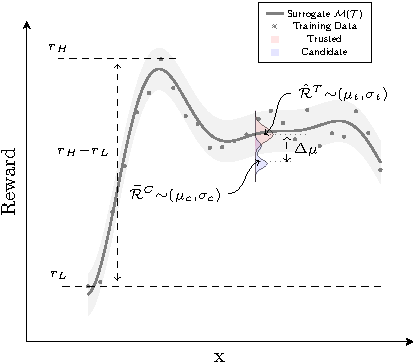
\includegraphics[width=0.95\linewidth]{Figures/xQ_v2.pdf}
    \caption{Key values for computing \xQ, where $x$ is a `feature of interest' for \task or \solve.}
    \label{fig:sq_v3}
    \vspace{-0.5cm}
\end{figure}

\begin{figure}[tbp]
    \centering
    \begin{subfigure}[c]{0.50\linewidth}
        \centering
        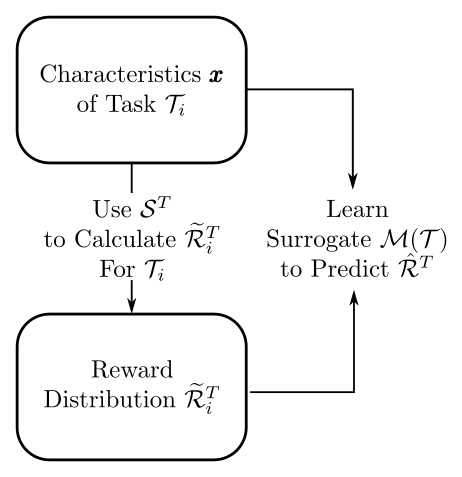
\includegraphics[width=0.75\linewidth]{Figures/xQ_train.png}
        \vfill
        \caption{Offline Training}
        \label{fig:xQ_train}
    \end{subfigure}%
    \hfill
    \begin{subfigure}[c]{0.50\linewidth}
        \centering
        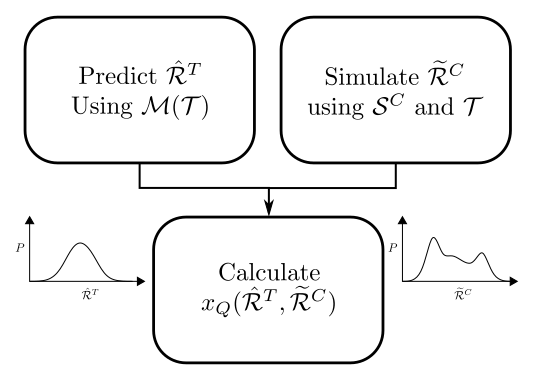
\includegraphics[width=0.75\linewidth]{Figures/xQ_test.png}
        \caption{Online Deployment}
        \label{fig:sQ_test}
    \end{subfigure} 
    \caption{Depiction of the training phase of the surrogate function \surrogate, and the test, or online deployment, phase where \xQ{} is calculated.}
    \label{fig:xQ_test_train}
    \vspace{-0.5cm}
\end{figure}

A surrogate model \surrogate{}, as shown in Fig.~\ref{fig:sq_v3} (right), can be learned in order to make a prediction \rwdtrustpredict{} of \rwdtrust{} from the `trusted' reference solver \solvetrust{} on task \task{} (ideally \solvetrust{} produces $\policytrust \approx \policy$ or converges to it with unlimited computing resources). The candidate solver \solvecand{} (which produces \policycand) must then be evaluated online with respect to the trusted solver \solvetrust{}. This is done by comparing \rwdtrustpredict{} and $\rwdcandsim= \ppicand$ (the simulated reward distribution of solver \solvecand{} on task \task). 

This approach is inspired by empirical hardness modeling techniques \cite{Leyton-Brown2009-yr}, which use surrogate models to predict the actual run time of NP-complete problem solvers. 
Figure~\ref{fig:sq_v3} (left) illustrates some of the key quantities involved in calculating \xQ{}. The basic premise is to evaluate a scaled version of the Hellinger distance between the difference between \rwdtrust{} and \rwd{}---the reward distributions of the trusted and candidate solvers respectively---while taking into account the overall range of rewards of the trusted solver over many tasks. 

The \emph{Hellinger Metric}, \hell{},  is a measure of the distance between two distributions. It is bounded between 0 and 1, where 0 means the distributions are identical. The maximum distance, 1, is achieved when one distribution $P$ assigns zero probability at every point in which another distribution $Q$ assigns probability. \hell{} has different forms based on the type of analytical distributions being compared. For the purposes of calculating \xQ{} from two distributions $P \sim (\mu_1,\sigma_1)$ and $Q\sim(\mu_2,\sigma_2)$ the following form is useful:
\begin{align}
    \hellmet &= 1-\sqrt{\frac{2\sigma_P\sigma_Q}{\sigma_P^2+\sigma_Q^2}}\exp{\left(-\frac{1}{4}\frac{(\mu_P-\mu_Q)^2}{\sigma_P^2+\sigma_Q^2}\right)} \\
    \text{q} &= \text{sgn}(\dmu)f^{\alpha}\sqrt{H^{2}(\rwdtrust,\rwd)} \label{eq:q}
\end{align}
Using \hell{} the overlap between the reward distributions \rwdtrustpredict{} and \rwdcandsim{} can be calculated. $\dmu= \mu_c-\mu_t$, and $f = \dmu/(r_H-r_L)$. The quantities $r_H$ and $r_L$ are largest and smallest $R_{\infty}$ values observed in the \surrogate{} training set. The exponent $\alpha$ is a parameter that affects the influence that $f$ has with respect to \hell (in essence, should the relationship of the effects of $f$ and \hell{} be $1:1$?). In practice $\alpha=1$ does not yield desirable results. \hell{} should be more influential on $\text{q}$ as $f$ grows smaller, and less influential as $f$ grows. We have found $\alpha=1/2$ gives results that `make sense'; future work could investigate the `best' value for $\alpha$ via user studies.

Similar to Eq.~\ref{eq:upm_lpm} the quantity $q$ is also unbounded above $0$ because while \hell{} is on the domain $[0,1]$, $f$ is on $[0,\infty)$. Consequently, as with \xO{}, a logistic function is used to keep the reported \xQ{}, shown in Eq.~\ref{eq:xQ}, value within some bounded range and avoid arbitrarily large values that can be confusing to humans. The numerator is 2 so that when $q=0$ (distributions are identical) \xQ{} will be 1. Dividing the quantity $q$ by 5 makes it so that \xQ{} `saturates' at around $\text{q}=\pm1$.
    \begin{align}
        \xQ &= \frac{2}{1+exp(-\text{q}/5)}\label{eq:xQ}
    \end{align}

Several numerical experiments are reported in \cite{Israelsen2018-qz} (\brett{this isn't anonymous}) to show that \xQ{} performs as expected in different situations. One of them is summarized here for illustrative purposes. Figure~\ref{fig:sq_thry1} illustrates the expected reward (with uncertainty) for a trusted solver \solvetrust{} given a specific, generic, task/solver parameter, as well as that of a `candidate' solver \solvecand. Different points of interest (indicating specific values of the task parameter) are highlighted by a star. The table on the side shows the values of \xQ{} calculated for different cases. At point B the candidate solver has a lower expected reward than the trusted solver and a higher variance than the trusted solver. Intuitively \xQ{} should be less than one. As shown when $r=5$ (i.e. $r_H-r_L=5$, the global reward range is `large') $x_Q=0.667$ which indicates that the candidate solver is marginally less capable than the trusted solver, and when $r=0.05$ then $x_Q=0.002$ indicates that \solvecand{} is much less capable than \solvetrust. At point C, \solvecand{} has higher expected reward than \solvetrust, but a larger variance. Intuitively expect \xQ{} of \solvecand{} to be a little greater than one; in fact when $r=5$, $x_Q=1.095$. As the global reward range $r$ decreases the difference in capability between \solvecand{} and \solvetrust{} increases with $x_Q=1.995$ at $r=0.005$. These calculations indicate that \xQ{} performs as expected.
\begin{figure}[tbp]
    \centering
    \begin{subfigure}[c]{0.5\linewidth}
        \centering
        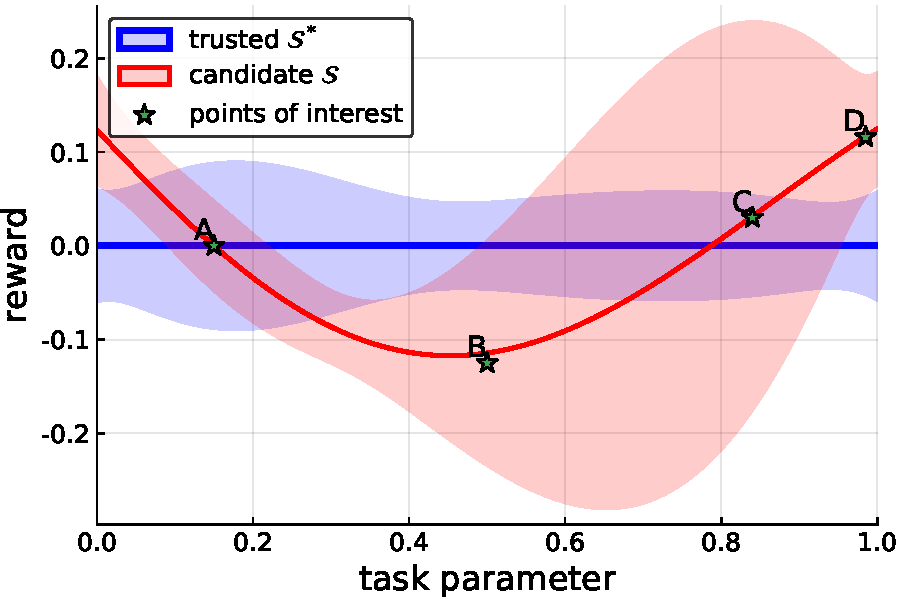
\includegraphics[width=0.99\linewidth]{Figures/p1.pdf}
        \vfill
    \end{subfigure}%
    \hfill
    \begin{subfigure}[t]{0.5\linewidth}
        \centering
        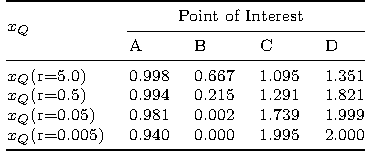
\includegraphics[width=0.95\linewidth]{Figures/p1_table.pdf}
    \end{subfigure} 
    \caption{\xQ{} from synthetic \pri{} pdfs for \solvetrust{} and \solvecand{}.}
    \label{fig:sq_thry1}
\end{figure}

\subsection{Contrast \xQ{} and \xO{}: Some Intuition}
The quantities \xQ{} and \xO{} are subtly different from each other. Perhaps a clarifying analogy can help to give an intuitive sense of the difference between the two. One could informally think of \xQ{} as an indication of the \emph{ability} of an athlete. This is opposed to the athlete's assessment of the desirability of the outcome of a game (\xO). While an athlete may be very capable (high \xQ), the score of the game may be such that the athlete knows that it is nearly impossible to catch up and win the game (low \xO). Conversely, an athlete may not be very capable (low \xQ), and due to being na\"{i}ve has an incorrect assessment of the desirability of the outcome (\xO{} cannot be trusted).
\brett{revisit this at the end}
